We also present the qualitative results, i.e. the fused images and some samples of each dataset. With the results from our IQA method, we have selected the eligible slices in each dataset and registered with the TrakEM2 alignment tool. The \textit{Callisia} dataset has six slices which present slight differences between the background of the leaf and the stomata. The images in this dataset are the brightest among all images in our datasets. Two eligible slices were obtained in the \textit{Tradescantia} dataset due to its large magnification, where either background sections or stomata are focused. Also, images in this dataset are not as bright as \textit{Callisia} ones, as the specimens present a strong purple color in their abaxial region. Finally, the \textit{Cthenante} dataset presents the strongest difference in focused regions among all datasets and also the darkest images. \autoref{fig:registered_slices} depicts samples of registered images in each dataset. 

\begin{figure}[ht]
    \centering
    \caption{Registered slices of our \textit{Callisia} (a), \textit{Tradescantia} (b) and \textit{Cthenante} (c) datasets.}
    \label{fig:registered_slices}
    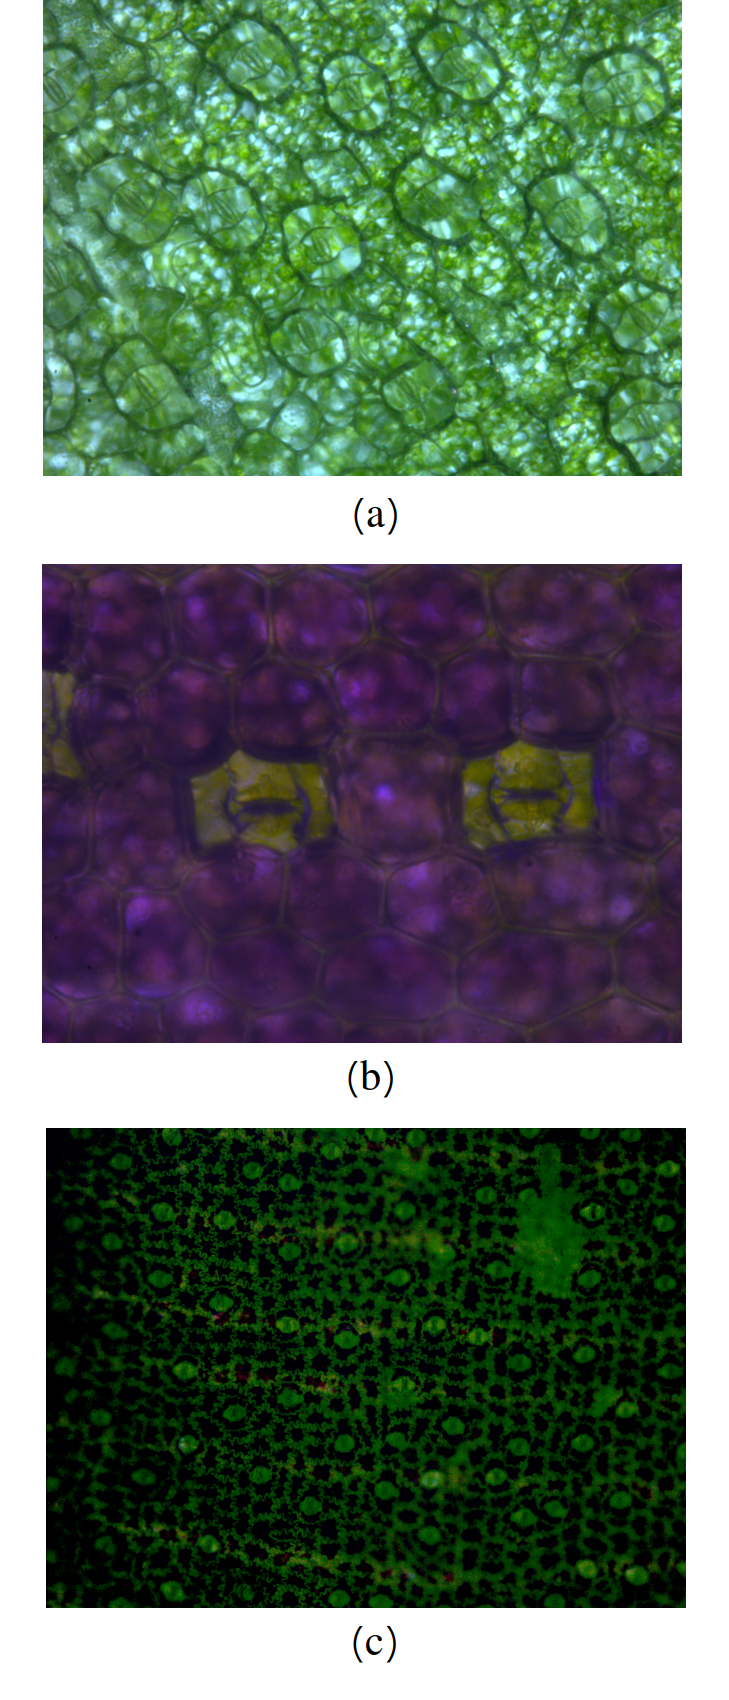
\includegraphics[scale=.32]{images/middle_images.png} \centering
    \fautor
\end{figure}

Each of the images in \autoref{fig:registered_slices} represent the middle of the z-stack. For example, \autoref{fig:registered_slices}.(c) is blurred on the left and right parts and sharp in the middle section; this shows that the leaf has a slope structure that promoted a clear division between blurred and sharp regions. The results of the fusion process of \textit{Callisia}, \textit{Tradescantia} and \textit{Cthennante} are shown in \autoref{fig:fused_callisia}, \autoref{fig:fused_tradescantia} and \autoref{fig:fused_cthenante}, respectively.

\begin{figure}[H]
  \centering
  \caption{Fused \textit{Callisia} image.}
  \label{fig:fused_callisia}
  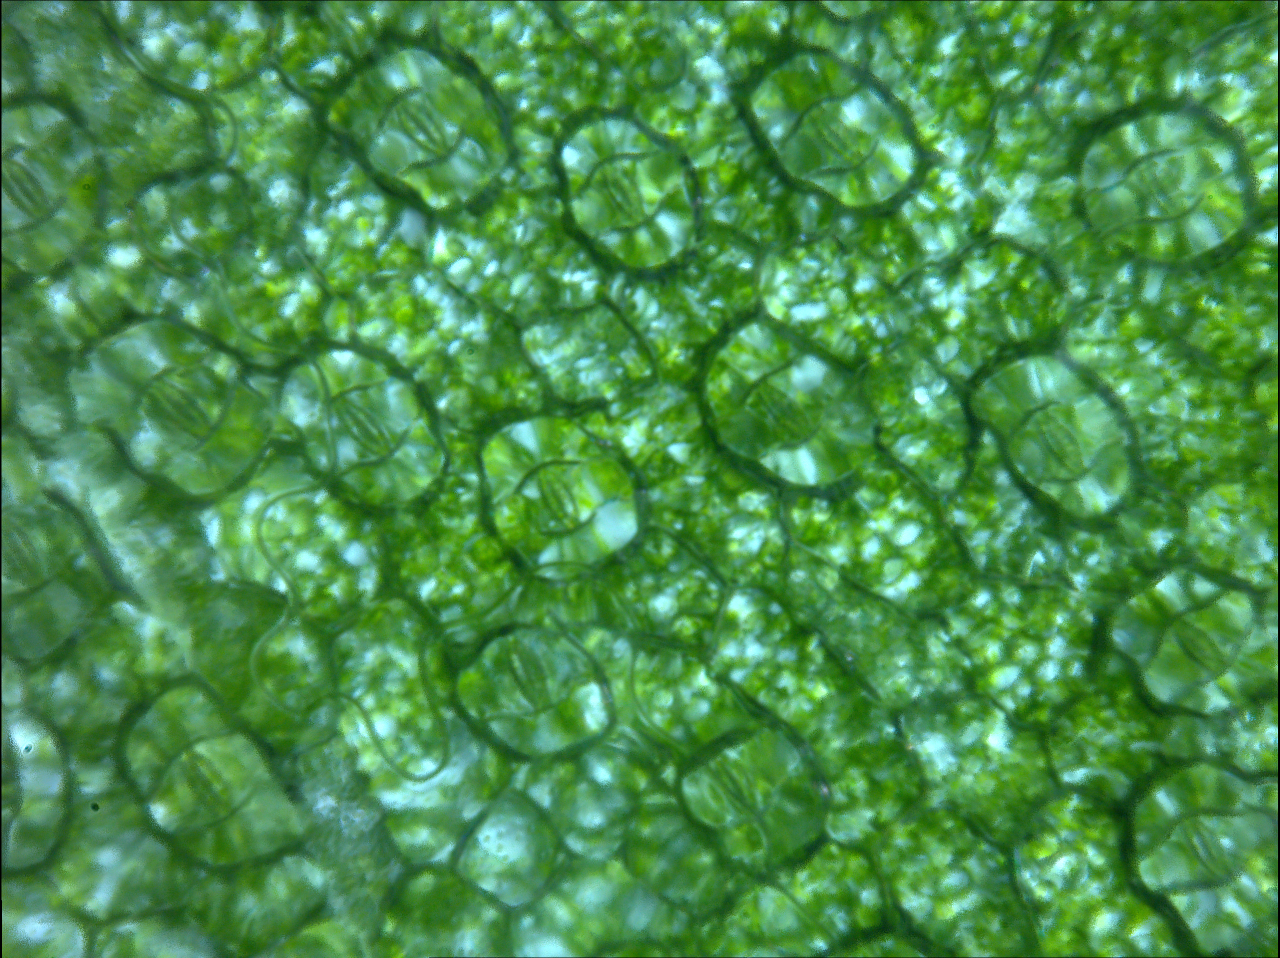
\includegraphics[scale=0.3]{images/fused_callisia.png}
  \centering
  \fautor
\end{figure}

\begin{figure}[H]
    \centering
    \caption{Fused \textit{Tradescantia} image.}
    \label{fig:fused_tradescantia}
    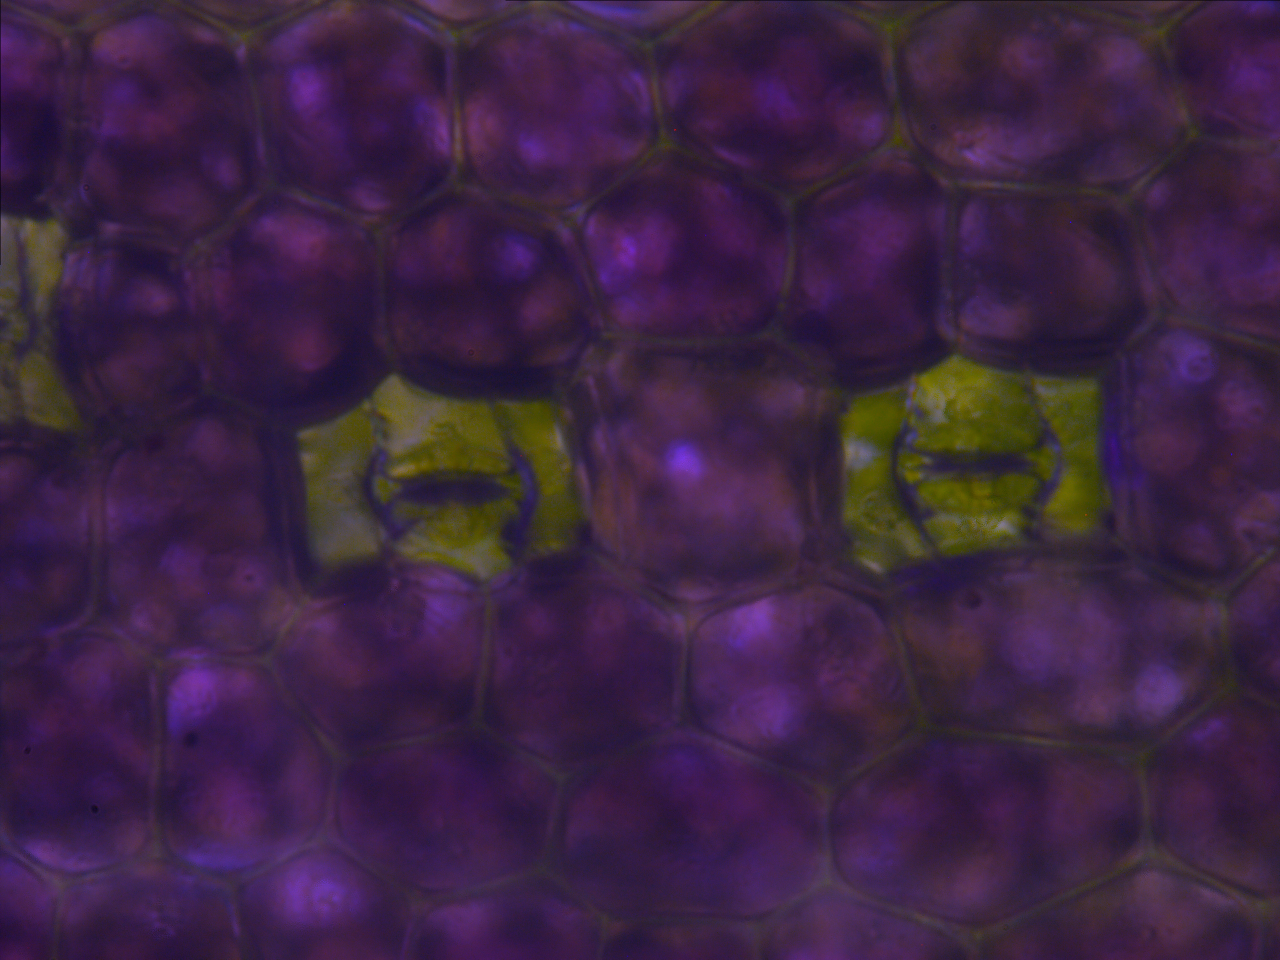
\includegraphics[scale=0.3]{images/fused_tradescantia.png}
    \centering
    \fautor
\end{figure}

\begin{figure}[H]
  \centering
  \caption{Fused \textit{Cthenante} image.}
  \label{fig:fused_cthenante}
  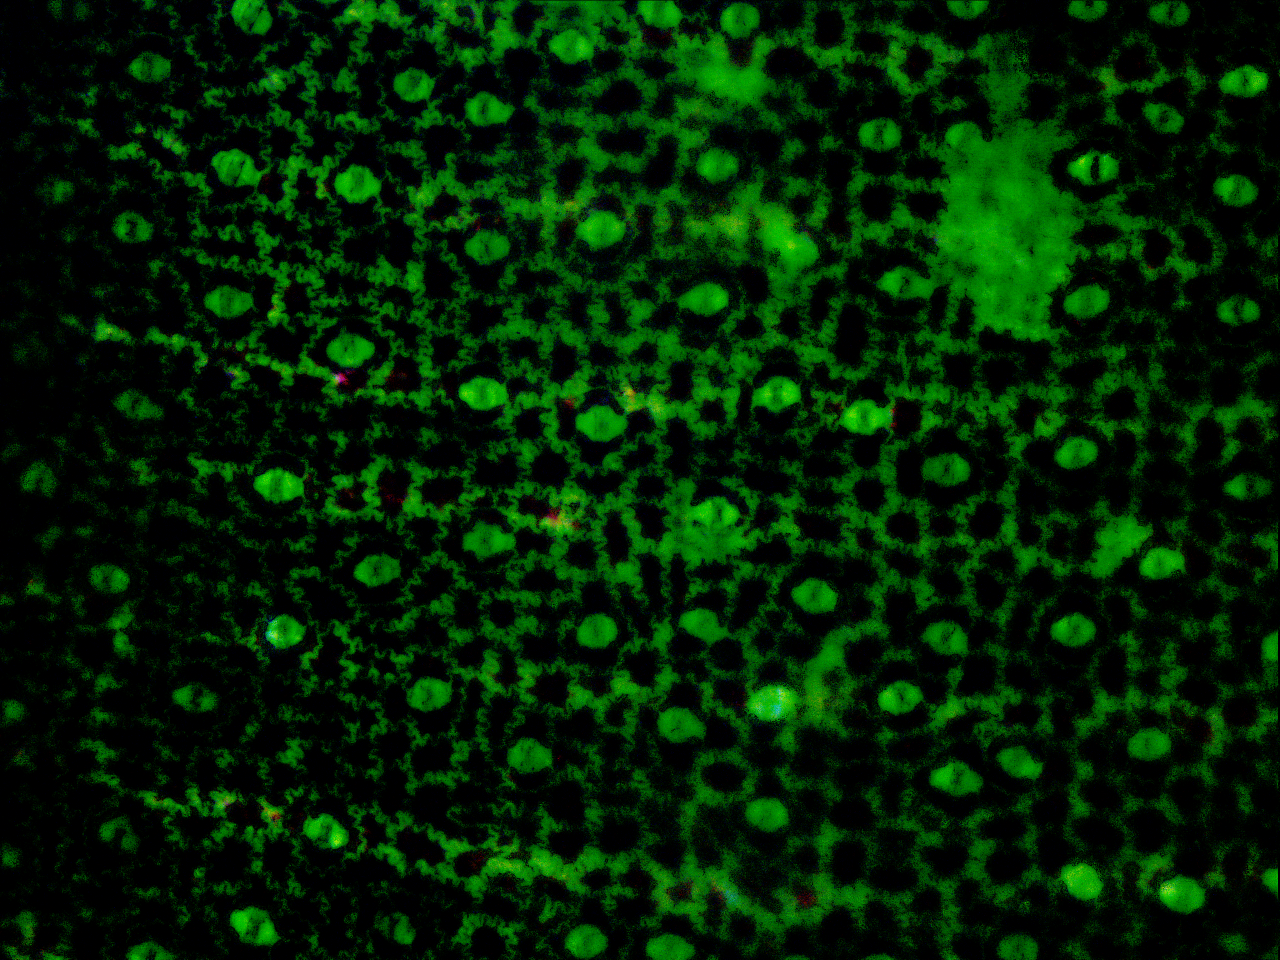
\includegraphics[scale=0.3]{images/fused_cthenante.png}
  \centering
  \fautor
\end{figure}